\documentclass[a4paper,11pt]{book}
%\documentclass[a4paper,twoside,11pt,titlepage]{book}
\usepackage{listings}
\usepackage[utf8]{inputenc}
\usepackage[spanish]{babel}
\usepackage{float}

% \usepackage[style=list, number=none]{glossary} %
%\usepackage{titlesec}
%\usepackage{pailatino}

\decimalpoint
\usepackage{dcolumn}
\newcolumntype{.}{D{.}{\esperiod}{-1}}
\makeatletter
\addto\shorthandsspanish{\let\esperiod\es@period@code}
\makeatother


%\usepackage[chapter]{algorithm}
\RequirePackage{verbatim}
%\RequirePackage[Glenn]{fncychap}
\usepackage{fancyhdr}
\usepackage{graphicx}
\usepackage{afterpage}
\usepackage{array}
\usepackage{makecell}
\usepackage{tabularray}
\usepackage{vcell}
\usepackage{booktabs}
\usepackage{textgreek}
\usepackage{amsmath} %Para poder usar \being{equation*}
\usepackage[gen]{eurosym} %Para usar el simbolo del euro en entornos varios 

\usepackage{longtable}

\usepackage[pdfborder={000}]{hyperref} %referencia

\usepackage[backend=biber, style=numeric, sorting=ynt]{biblatex}


% \usepackage{booktabs}
% \usepackage{dirtree}
% \usepackage{algorithmicx}
% \usepackage{algorithm}
\usepackage[font=small, margin=0.1cm]{caption}
% \usepackage{subcaption}
\usepackage{multirow}
% \usepackage{enumitem}
% \setlist{nosep}

\newcommand{\INDSTATE}[1][1]{\STATE\hspace{#1\algorithmicindent}}

% \usepackage[
%     a4paper,
%     left=2.8cm,
%     right=2.7cm,
%     top=4cm,
%     bottom=3cm
% ]{geometry}

% ********************************************************************
% Re-usable information
% ********************************************************************
\newcommand{\myTitle}{Detección de errores en bases de datos químicas\xspace}
\newcommand{\myDegree}{Grado en Ingeniería Informática\xspace}
\newcommand{\myName}{Jesús Navarro Merino\xspace}
\newcommand{\myProf}{Rocío Celeste Romero Zaliz\xspace}
%\newcommand{\mySupervisor}{Put name here\xspace}
\newcommand{\myFaculty}{Escuela Técnica Superior de Ingenierías Informática y de
Telecomunicación\xspace}
\newcommand{\myFacultyShort}{E.T.S. de Ingenierías Informática y de
Telecomunicación\xspace}
\newcommand{\myDepartment}{Departamento de ...\xspace}
\newcommand{\myUni}{\protect{Universidad de Granada}\xspace}
\newcommand{\myLocation}{Granada\xspace}
\newcommand{\myTime}{\today\xspace}
\newcommand{\myVersion}{Version 0.1\xspace}


\hypersetup{
pdfauthor = {\myName (email (en) ugr (punto) es)},
pdftitle = {\myTitle},
pdfsubject = {},
pdfkeywords = {palabra_clave1, palabra_clave2, palabra_clave3, ...},
pdfcreator = {LaTeX con el paquete ....},
pdfproducer = {pdflatex}
}

%\hyphenation{}


%\usepackage{doxygen/doxygen}
%\usepackage{pdfpages}
\usepackage{url}
\usepackage{color,colortbl,longtable}
\usepackage{tabularx}
\usepackage{lscape}
\usepackage[stable]{footmisc}
%\usepackage{index}

%\makeindex
%\usepackage[style=long, cols=2,border=plain,toc=true,number=none]{glossary}
% \makeglossary

% Definición de comandos que me son tiles:
%\renewcommand{\indexname}{Índice alfabético}
%\renewcommand{\glossaryname}{Glosario}

\pagestyle{fancy}
\fancyhf{}
\fancyhead[LO]{\leftmark}
\fancyhead[RE]{\rightmark}
\fancyhead[RO,LE]{\textbf{\thepage}}
\renewcommand{\chaptermark}[1]{\markboth{\textbf{#1}}{}}
\renewcommand{\sectionmark}[1]{\markright{\textbf{\thesection. #1}}}

\setlength{\headheight}{1.5\headheight}

\newcommand{\HRule}{\rule{\linewidth}{0.5mm}}
%Definimos los tipos teorema, ejemplo y definición podremos usar estos tipos
%simplemente poniendo \begin{teorema} \end{teorema} ...
\newtheorem{teorema}{Teorema}[chapter]
\newtheorem{ejemplo}{Ejemplo}[chapter]
\newtheorem{definicion}{Definición}[chapter]

\definecolor{gray97}{gray}{.97}
\definecolor{gray75}{gray}{.75}
\definecolor{gray45}{gray}{.45}
\definecolor{gray30}{gray}{.94}

\lstset{ frame=Ltb,
     framerule=0.5pt,
     aboveskip=0.5cm,
     framextopmargin=3pt,
     framexbottommargin=3pt,
     framexleftmargin=0.1cm,
     framesep=0pt,
     rulesep=.4pt,
     backgroundcolor=\color{gray97},
     rulesepcolor=\color{black},
     %
     stringstyle=\ttfamily,
     showstringspaces = false,
     basicstyle=\scriptsize\ttfamily,
     commentstyle=\color{gray45},
     keywordstyle=\bfseries,
     %
     numbers=left,
     numbersep=6pt,
     numberstyle=\tiny,
     numberfirstline = false,
     breaklines=true,
   }
 
% minimizar fragmentado de listados
\lstnewenvironment{listing}[1][]
   {\lstset{#1}\pagebreak[0]}{\pagebreak[0]}

\lstdefinestyle{CodigoC}
   {
	basicstyle=\scriptsize,
	frame=single,
	language=C,
	numbers=left
   }
\lstdefinestyle{CodigoC++}
   {
	basicstyle=\small,
	frame=single,
	backgroundcolor=\color{gray30},
	language=C++,
	numbers=left
   }

 
\lstdefinestyle{Consola}
   {basicstyle=\scriptsize\bf\ttfamily,
    backgroundcolor=\color{gray30},
    frame=single,
    numbers=none
   }


\newcommand{\bigrule}{\titlerule[0.5mm]}


%Para conseguir que en las páginas en blanco no ponga cabecerass
\makeatletter
\def\clearpage{%
  \ifvmode
    \ifnum \@dbltopnum =\m@ne
      \ifdim \pagetotal <\topskip
        \hbox{}
      \fi
    \fi
  \fi
  \newpage
  \thispagestyle{empty}
  \write\m@ne{}
  \vbox{}
  \penalty -\@Mi
}
\makeatother

\usepackage{pdfpages}


\addbibresource{bibliografia/bibliografia.bib}
% \addbibresource{sample.bib}
% \addbibresource{bibliografia/webs.bib}

\begin{document}
\begin{titlepage}
 
 
\newlength{\centeroffset}
\setlength{\centeroffset}{-0.5\oddsidemargin}
\addtolength{\centeroffset}{0.5\evensidemargin}
\thispagestyle{empty}

\noindent\hspace*{\centeroffset}\begin{minipage}{\textwidth}

\centering

\includegraphics[width=0.9\textwidth]{imagenes/logos/logo_ugr.jpg}\\[1.4cm]

\textsc{ \Large TRABAJO FIN DE GRADO\\[0.2cm]}
\textsc{ INGENIERÍA INFORMÁTICA}\\[1cm]
% Upper part of the page
% 
% Title
\noindent\rule[-1ex]{\textwidth}{2pt}\\[3ex]
{\Huge\bfseries Prueba Detección de errores en bases de datos químicas\\
}
\noindent\rule[-3ex]{\textwidth}{2pt}\\[3ex]
\end{minipage}

\vspace{1.5cm}
\noindent\hspace*{\centeroffset}\begin{minipage}{\textwidth}
\centering

\textbf{Autor}\\ {Jesús Navarro Merino}\\[2.5ex]
\textbf{Directora}\\
{Rocío Celeste Romero Zaliz}\\[2cm]

\includegraphics[width=0.3\textwidth]{imagenes/logos/etsiit_logo.png}\\[0.1cm]
\textsc{Escuela Técnica Superior de Ingenierías Informática y de Telecomunicación}\\
\textsc{---}\\
Granada, julio de 2023
\end{minipage}
%\addtolength{\textwidth}{\centeroffset}
%\vspace{\stretch{2}}
\end{titlepage}


\chapter*{}
%\thispagestyle{empty}
%\cleardoublepage

%\thispagestyle{empty}


% \cleardoublepage
\thispagestyle{empty}

\begin{center}
{\large\bfseries Detección de errores en bases de datos químicas}\\
\end{center}
\begin{center}
Jesús Navarro Merino\\
\end{center}

%\vspace{0.7cm}
\noindent{\textbf{Palabras clave}: Química computacional, Química organometálica, Nomenclatura canónica, SMILES, Representación de moléculas, Cp, OpenBabel, Bases de datos, SciFinder.}\\

\vspace{0.7cm}
\noindent{\textbf{Resumen}}\\

El desarrollo de la informática y la aplicación de sus métodos al mundo de la química ha propiciado grandes avances en esta ciencia. Sin embargo, un campo poco explorado dentro de la química computacional es la organometálica, de manera que muchas de las herramientas existentes no están preparadas para trabajar con ella. En esta área, para los investigadores es importante codificar las moléculas en representaciones lineales como SMILES y usar las herramientas software, para entre otras cosas, representar los compuestos gráficamente y comprenderlos mejor. La heterogeneidad en las distintas bases de datos públicas a la hora de consultar un mismo compuesto entorpece el trabajo de los investigadores.

Tras un análisis de esas inconsistencias, este proyecto propone una nomenclatura canónica para moléculas organometálicas en donde se le dé la suficiente importancia al metal, de manera que quede colocado el primero en el SMILES canónico resultado. En química de coordinación y organometálica, las reacciones y los compuestos no se explican bien siguiendo la teoría del enlace de valencia. Por tanto, se presentan también algunos cambios en el sistema de representación 2D de la herramienta utilizada, para ilustrar de una manera más adecuada los enlaces metal-ligando más habituales en compuestos organometálicos, las estructuras de ciclopentadienilo (Cp). Tras la validación de los resultados con diversos tests de consistencia, se obtienen finalmente resultados satisfactorios.

\cleardoublepage


\thispagestyle{empty}


\begin{center}
{\large\bfseries Error detection in chemical databases}\\
\end{center}
\begin{center}
Jesús Navarro Merino\\
\end{center}

%\vspace{0.7cm}
\noindent{\textbf{Keywords}: Chemoinformatics, Organometallic chemistry, Canonicalization, SMILES, Molecule depiction, Cp, OpenBabel, Databases, SciFinder.}\\

\vspace{0.7cm}
\noindent{\textbf{Abstract}}\\

The development of computer science and the application of its methods to the chemical world has led to great advances in this science. However, a less explored field within computational chemistry is organometallics, meaning that many of the existing tools are not prepared to work with it. In this area, it is important for researchers to encode molecules in linear notations such as SMILES and use software tools to, among other things, depict compounds graphically and have a better understanding of them. Heterogeneity in various public databases when querying the same compound hinders scientists' work.

After an analysis of these inconsistencies, this project proposes a canonical nomenclature for organometallic molecules in which adequate importance is given to the metal, so that it is placed first in the resulting canonical SMILES. In coordination and organometallic chemistry, reactions and compounds do not fit well into the valence bond theory. Therefore, some changes are also presented in the 2D representation system of the tool used, in order to illustrate in a more suitable way the most common metal-ligand bonds in organometallic compounds, cyclopentadienyl (Cp) complexes. After validation of the results with several consistency tests, satisfactory outcomes are finally obtained.

\chapter*{}
\thispagestyle{empty}

\noindent\rule[-1ex]{\textwidth}{2pt}\\[4.5ex]

Yo, \textbf{Jesús Navarro Merino}, alumno de la titulación Grado en Ingeniería Informática de la \textbf{Escuela Técnica Superior
de Ingenierías Informática y de Telecomunicación de la Universidad de Granada}, con DNI 15429457E, autorizo la
ubicación de la siguiente copia de mi Trabajo Fin de Grado en la biblioteca del centro para que pueda ser
consultada por las personas que lo deseen.

\vspace{6cm}

\noindent Fdo: Jesús Navarro Merino

\vspace{2cm}

\begin{flushright}
Granada, a 11 de julio de 2023
\end{flushright}


\chapter*{}
\thispagestyle{empty}

\noindent\rule[-1ex]{\textwidth}{2pt}\\[4.5ex]

Dña. \textbf{Rocío Celeste Romero Zaliz}, Profesora del Departamento de Ciencias de la Computación e Inteligencia Artificial de la Universidad de Granada.


\vspace{0.5cm}

\textbf{Informan:}

\vspace{0.5cm}

Que el presente trabajo, titulado \textit{\textbf{Detección de errores en bases de datos químicas}},
ha sido realizado bajo su supervisión por \textbf{Jesús Navarro Merino}, y autorizamos la defensa de dicho trabajo ante el tribunal que corresponda.

\vspace{0.5cm}

Y para que conste, expiden y firman el presente informe en Granada a 11 de julio de 2023.

\vspace{1cm}

\textbf{La directora:}

\vspace{5cm}

\noindent \textbf{Rocío Celeste Romero Zaliz}

\chapter*{Agradecimientos}
\thispagestyle{empty}

       \vspace{1cm}


A mi tutora Rocío, por su esfuerzo y guía a lo largo del proyecto. Por su paciencia y ánimos en los momentos más críticos.
\\

A mis amigos, que por los buenos momentos vividos y el día a día con ellos, han hecho que estos años en la universidad hayan pasado casi sin darme cuenta.
\\

Y a mis padres, por su apoyo incondicional y confianza durante todo este trayecto. 
\frontmatter
\tableofcontents
\listoffigures
\renewcommand{\listtablename}{Índice de tablas}
\renewcommand{\tablename}{Tabla}
\listoftables

\mainmatter
\setlength{\parskip}{5pt}

% --------------------------------------Capítulos-----------------------------
\chapter{Introducción}




% \begin{tblr}{|Q[h,t]|Q[c,t]|Q[r,b]|}
% \hline
% {C[Au].c1ccc(cc1)P(c2ccccc2)c3ccccc3 \\ Left Left} & Middle Center & {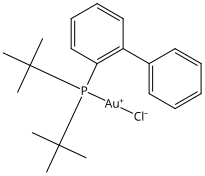
\includegraphics{imagenes/SciFinder/Chloro[(1,1-biphenyl-2-yl)di-tert-butylphosphine]gold(I).png}} \\
% \hline
% \end{tblr}

\textbf{Meter aqui una introduccion general sobre la química, la quimica informatica (y cómo surge en base a las necesidades computacionales), mencionar brevemente la organometalica (mas tarde en la seccion de estado del arte profundizo, junto con cosas de dibujado, tutorial de SMILES, y representacion de moléculas)}


\section{Motivación y objetivos}

Los formatos de notación lineal llevan siendo un tema de interés e investigación para los científicos desde mediados del siglo 19 \cite{107_years_linear_notations} \textbf{Terminar esto}

En la actualidad, existen varias representaciones lineales \textbf{(Para esto debo haber hablado antes de las representaciones lineales, o bien lo explico aquí, o bien lo redirijo a los fundamentos teóricos. O bien, justo antes de empezar este párrafo, que será lo mejor-> quitar entonces la siguiente negrita)}, siendo las más usadas SMILES, InChI, y SELFIES \cite{SELFIES}. \textbf{Como comenté antes, una forma muy potente de representar moléculas y compuestos químicos es mediante cadenas strings}, y de esto justamente se encargan las representaciones lineales: traducir una molécula, con sus átomos, enlaces entre ellos, ciclos y otras propiedades características, en una cadena string que la represente, y que la máquina y los propios químicos puedan entender. Sin embargo, hay diferencias notables entre las representaciones, tanto en la sintaxis de las cadenas que se generan como en las aplicaciones que se le puede dar a cada una de ellas.

SMILES, ideada por David Weininger, sale a la luz en 1988 satisfaciendo con creces las necesidades de procesamiento de información química que había, desbancando a la representación estandarizada del momento, Wiswesser Line Notation (WLN). Desde ese entonces SMILES se convirtió —y sigue siendo a día de hoy— en el estándar de representación lineal, ya que permite describir estructuras moleculares de una forma sencilla en un formato fácil de leer, lo que ha hecho que sea una herramienta popular en la química computacional, siendo la más usada entre investigadores y químicos. Pese a esto, SMILES tiene dos grandes inconvenientes: una misma molécula puede escribirse con varias cadenas SMILES distintas válidas, es decir, tiene sinónimos (Figura \ref{fig:sinonimos_smiles}); y no es robusto ni sintáctica ni semánticamente. En este sentido se podría generar un string que no represente una molécula válida, como lo es \emph{CC(CCCC}, el cual tiene un paréntesis sin cerrar (lo que implica que no se delimita cuándo acaba la rama). O generar una molécula que no sea químicamente viable como \emph{CO=CC}, que muestra un átomo de oxígeno neutro formando tres enlaces (superando el límite de enlaces covalentes que un oxígeno neutro puede tener) \cite{SELFIES}.

\begin{figure}[H]
\centering
    \fbox{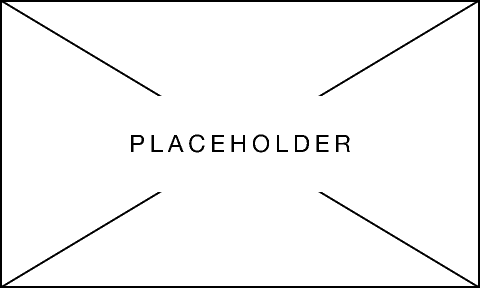
\includegraphics[scale=0.3]{imagenes/placeholder.png}}  
    \caption{Distintas cadenas SMILES válidas para la misma molécula de <nombre-molecula>. \cite{}}
    \label{fig:sinonimos_smiles}
\end{figure}

Esto tiene especial relevancia en el ámbito del Machine Learning (ML). Aunque se sale del alcance de este trabajo, uno de los grandes objetivos de la química computacional es la creación o diseño de nuevas moléculas. Se podrían crear modelos de ML o redes neuronales capaces de generar moléculas ficticias válidas, para posteriormente ver sus propiedades, valorarlas energéticamente para ver cuán estables son, y estudiar su viabilidad en distintas aplicaciones, entre otras cosas. SMILES dificulta esta tarea, y por ello, aparece en 2020, SELFIES (SELF-referencIng Embedded Strings), una nueva representación lineal 100\% robusta, muy usada actualmente para modelos generativos. Ver \cite{SELFIES, krenn_self_referencing_2020} para más detalles de cómo soluciona los problemas de robustez y otras características de la representación. SELFIES es relativamente reciente y continuamente está ampliando sus funcionalidades, mejorando su simplicidad y facilidad de uso para el usuario \cite{selfies_recent_2023}. Aun así, no se termina de instaurar entre la comunidad investigadora. 

\textbf{AQUI METER ALGO DE InChI, o lo meto arriba, antes de hablar sobre SELFIES.
}

Por todo lo anterior, me centraré en la notación SMILES durante el desarrollo de este trabajo. Dicho esto, existen diversas fuentes de datos en química donde se recoge gran cantidad de información acerca de los compuestos. Menciono las más importantes y las que serán objeto de interés. \emph{PubChem}, una base de datos abierta que sirve información a millones de usuarios en todo el mundo, desde investigadores y estudiantes hasta el público general. Recogen para cada compuesto, información sobre su estructura, representaciones 2D y 3D, identificadores, propiedades químicas y físicas, patentes, avisos de toxicidad, etc. \cite{pubchem_website} 

\emph{SciFinder}, una herramienta de investigación muy potente que permite explorar las bases de datos de CAS (American Chemical Society) las cuales contienen literatura sobre Química y otras disciplinas afines como Física, Biomedicina, Geología, Ingeniería Química, etc. Incluye referencias bibliográficas y resúmenes de artículos, informes, y libros entre otras cosas. Permite realizar búsquedas por estructura, nombres de sustancias o identificadores, reacciones en la que participa dicha sustancia, artículos y publicaciones que nombren el compuesto en cuestión, e incluso proveedores de compra. Para el uso de esta herramienta es necesario acceder mediante la red de una institución autorizada (en este caso trabajo mediante VPN de la UGR) y seguir los pasos para registrarte \footnote{Pasos para el registro en SciFinder \url{https://bibliotecaugr.libguides.com/scifinder_scholar}}

uno de los principales problemas que se detectan es la heterogeneidad en las distintas bases de datos \textbf{continuar esto}



\textbf{Aquí empezar ya con la tabla comparativa. Para eso, tengo que introducir las fuentes de datos }

\noindent \textbf{Meter parrafo de los quimicos colaboradores...mirar pedro}

Por todo lo anterior, una solución que permita aunar... \textbf{continuar esto}  

Por tanto, el objetivo principal de este Trabajo Fin de Grado sería modificar el paquete OpenBabel creando un método para canonizar códigos SMILES, orientado específicamente para compuestos organometálicos, de los cuales dispongo de un conjunto de datos de 30 moléculas considerados de interés por la tutora y los químicos con los que colabora. Para ello, se establecen los siguientes subobjetivos:
\begin{itemize}
    \item Analizar y comparar las cadenas SMILES de distintas bases de datos (p.ej. Sigma-Aldrich, SciFinder) viendo los posibles sinónimos para una misma molécula.
    \item Determinar un sistema que genere, a partir de cualquier sinónimo SMILES de la misma molécula, un único SMILES canónico.
    \item Definir otro algoritmo o conjunto de reglas que mejore, aunque sea mínimamente, el sistema de dibujado de los compuestos.
\end{itemize} 



\begin{table}
\small
  \begin{tabular}
      {lc} \hline Código SMILES & Representación 2D \\ \hline C[Au].c1ccc(cc1)P(c2ccccc2)c3ccccc3 & \parbox[c]{5em}{
      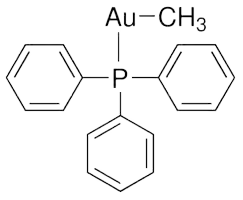
\includegraphics[width=2cm]{imagenes/SigmaAldrich/Methyl(triphenylphosphine)gold(I).png}} \\ \hline
      Cl[Pd]Cl.C1CC=CCCC=C1 & \parbox[r]{5em}{
      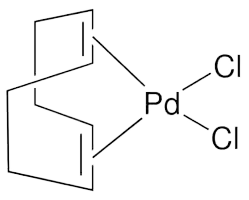
\includegraphics[width=2cm]{imagenes/SigmaAldrich/Dichloro(1,5-cyclooctadiene)palladium(II).png}} \\ \hline
      Cl[Au].CP(C)C & \parbox[c]{5em}{
      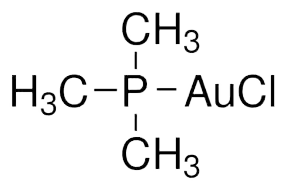
\includegraphics[width=2cm]{imagenes/SigmaAldrich/Chloro(trimethylphosphine)gold(I).png}} \\ \hline
      Cl[Au].CC(C)(C)P(c1ccccc1-c2ccccc2)C(C)(C)C & \parbox[c]{5em}{
      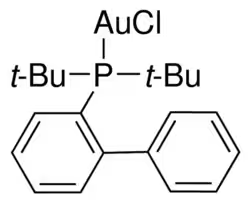
\includegraphics[width=2cm]{imagenes/SigmaAldrich/Chloro[(1,1-biphenyl-2-yl)di-tert-butylphosphine]gold(I).png}} \\ \hline
      [Fe]I.[C-]\#[O+].[C-]\#[O+].[CH]1[CH][CH][CH][CH]1 & \parbox[c]{5em}{
      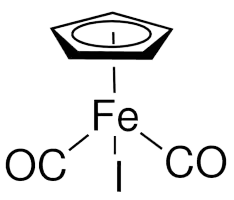
\includegraphics[width=2cm]{imagenes/SigmaAldrich/Dicarbonylcyclopentadienyliodoiron(II).png}} \\ \hline
  \end{tabular}
  \caption{Códigos SMILES y sus representaciones 2D según Sigma-Aldrich}
\end{table}


\begin{table}
\small
  \begin{tabular}
      {lc} \hline Código SMILES & Representación 2D \\ \hline 
      [Au+]([CH3-])[P](C=1C=CC=CC1)(C=2C=CC=CC2)C=3C=CC=CC3 & \parbox[c]{5em}{
      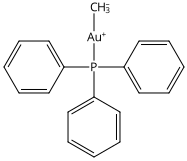
\includegraphics[width=2cm]{imagenes/SciFinder/Methyl(triphenylphosphine)gold(I).png}} \\ \hline
      [Cl-][Pd+2]123([Cl-])[CH]=4CC[CH]3=[CH]2CC[CH]41 & \parbox[r]{5em}{
      \includegraphics[width=2cm]{imagenes/SciFinder/Dichloro(1,5-cyclooctadiene)palladium(II).png}} \\ \hline
      [Cl-][Au+][P](C)(C)C & \parbox[c]{5em}{
      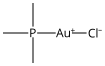
\includegraphics[width=2cm]{imagenes/SciFinder/Chloro(trimethylphosphine)gold(I).png}} \\ \hline
      [Cl-][Au+][P](C=1C=CC=CC1C=2C=CC=CC2)(C(C)(C)C)C(C)(C)C & \parbox[c]{5em}{
      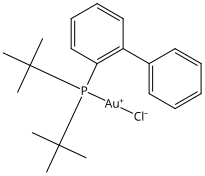
\includegraphics[width=2cm]{imagenes/SciFinder/Chloro[(1,1-biphenyl-2-yl)di-tert-butylphosphine]gold(I).png}} \\ \hline
      O\#C[Fe+2]1234([I-])(C\#O)[CH]=5[CH]4=[CH]3[CH-]2[CH]51 & \parbox[c]{5em}{
      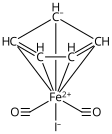
\includegraphics[width=2cm]{imagenes/SciFinder/Dicarbonylcyclopentadienyliodoiron(II).png}} \\ \hline
  \end{tabular}
  \caption{Códigos SMILES y sus representaciones 2D según SciFinder}
\end{table}








\begin{table}
  \begin{tblr}
      {Q[c,t]Q[c,m]} \hline Código SMILES & Representación 2D \\ \hline 
      C[Au].c1ccc(cc1)P(c2ccccc2)c3ccccc3 & 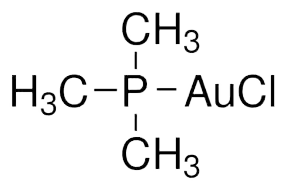
\includegraphics[width=2cm]{imagenes/SigmaAldrich/Chloro(trimethylphosphine)gold(I).png}
       \\
      Cl[Pd]Cl.C1CC=CCCC=C1 & 
      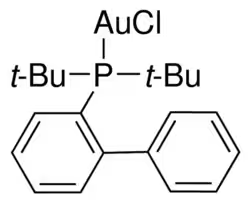
\includegraphics[width=2cm]{imagenes/SigmaAldrich/Chloro[(1,1-biphenyl-2-yl)di-tert-butylphosphine]gold(I).png} \\
      Cl[Au].CP(C)C & 
      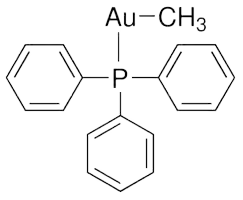
\includegraphics[width=2cm]{imagenes/SigmaAldrich/Methyl(triphenylphosphine)gold(I).png} \\
      Cl[Au].CC(C)(C)P(c1ccccc1-c2ccccc2)C(C)(C)C & 
      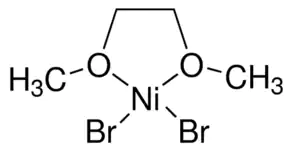
\includegraphics[width=2cm]{imagenes/SigmaAldrich/Nickel(II) bromide ethylene glycol dimethyl ether complex.png} \\ [0cm]
    [Fe]I.[C-]\#[O+].[C-]\#[O+].[CH]1[CH][CH][CH][CH]1 & 
      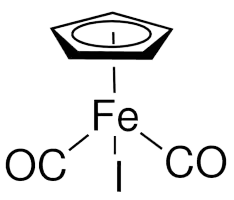
\includegraphics[width=2cm]{imagenes/SigmaAldrich/Dicarbonylcyclopentadienyliodoiron(II).png} \\ \hline
  \end{tblr}
  \caption{Códigos SMILES y sus representaciones 2D según Sigma-Aldrich}
\end{table}


% \begin{longtblr}{
%   colspec={Q[valign=t]Q[valign=b]Q[valign=h]},
%   row{1}={halign=c},
%   hlines
% }
% Id & Name & Figure \\
% 1 & Press imaginary a button & 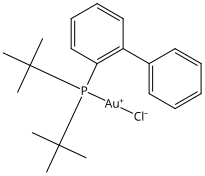
\includegraphics{imagenes/SciFinder/Chloro[(1,1-biphenyl-2-yl)di-tert-butylphosphine]gold(I).png}\\ 
% 1 & Press imaginary a button & 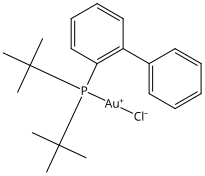
\includegraphics{imagenes/SciFinder/Chloro[(1,1-biphenyl-2-yl)di-tert-butylphosphine]gold(I).png}\\
% 1 & Press imaginary a button & 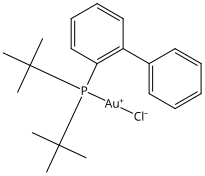
\includegraphics{imagenes/SciFinder/Chloro[(1,1-biphenyl-2-yl)di-tert-butylphosphine]gold(I).png}\\
% 1 & Press imaginary a button & 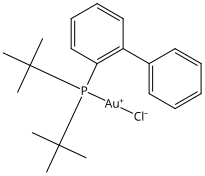
\includegraphics{imagenes/SciFinder/Chloro[(1,1-biphenyl-2-yl)di-tert-butylphosphine]gold(I).png}\\
% 1 & Press imaginary a button & 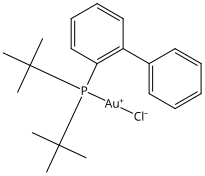
\includegraphics{imagenes/SciFinder/Chloro[(1,1-biphenyl-2-yl)di-tert-butylphosphine]gold(I).png}\\
% 1 & Press imaginary a button & 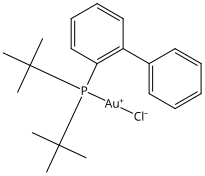
\includegraphics{imagenes/SciFinder/Chloro[(1,1-biphenyl-2-yl)di-tert-butylphosphine]gold(I).png}\\
% \end{longtblr}

\section{Objetivos}


\section{Estructura de la memoria}

% \begin{table}[ht]
%     \centering
%     \begin{tabular}{p{0.35\linewidth} | p{0.6\linewidth}}
%       Column 1  & Column2 \\ \hline
%       This text will be wrapped & Some more text \\
%       Some text here & This text maybe wrapped here if its tooooo long \\
%     \end{tabular}
%     \caption{Caption}
%     \label{tab:my_label}
% \end{table}


\chapter{Estado del arte y fundamentos teóricos}

Quizas sea mejor mover esta seccion justo despues de la introduccion para seguir con la tematica de la motivacion, y ya luego me meto con la gestion y planificacion

Puedo hacer una revision de la literatura existente hasta dia de hoy sobre el tema
Usar SCOPUS para esto, con terminos tipo: "SMILES" "molecule" "organometalic" (juntarlos o separarlos segun vea)

Hablar por aqui de la organometalica, representacion de moléculas, Hablar mas extendido de SMILES, SELFIES, e INCHI; cosas de dibujado de moleculas (los paquetes que hay), )
No se si meterlo aqui o en otro apartado, el diagrama de clases

la historia de la humanidad está marcada por la búsqueda de materiales que mejoren su calidad de vida, y los metales han sido parte crucial de esos cambios 

La materia que forma los seres vivos tiene en su composición sustancias cuya base I principal es el carbono. El estudio de estos compuestos constituye una rama de la química llamada química orgánica. La abundancia del carbono en el planeta es relativamente pequeña: aproximadamente un 0,03 \%; sin embargo, da lugar a millones de sustancias diferentes, mientras que los compuestos inorgánicos son solo unos pocos miles. ¿Qué hace a este elemento tan especial? Su estructura singular, que le permite formar largas cadenas en las cuales una pequeña variación da lugar a un compuesto distinto al anterior.


(del archivo de informeReuniones puedo ir sacando cosas para meter en el estado del arte) Openbabel como tal no soporta el dibujado en 3D de las moléculas, por lo que los únicos dibujos que puede hacer son en 2D. Openbabel tampoco soporta el uso de wedge ni hash bonds para el dibujado de moléculas en 2D con perspectiva (es curioso porque en el código sí que hay funciones dedicadas a esto, pero luego cuando le metes símbolos SMILES de @@ y demás, los medio ignora. Sigo ejemplos del tutorial de Daylight, pero no salen los mismos dibujos. Otros símbolos más dedicados a geometría que viene en Daylight o en OpenSMILES, tipo @SP, @TB, @OH, los ignora por completo). Pero sí es capaz de generar archivos .sdf con información 3D, que se pueden usar en otros softwares de dibujado específicos como Avogadro (y no están mal, mucho mejor que los 2D desde luego)

\bigskip

\chapter{Gestión y Planificación del proyecto}



\section{Metodología}


\section{Gestión de recursos}

\subsection{Recursos humanos}

\subsection{Recursos materiales}

\subsection{Recursos software}

\section{Gestión de costes}

\subsection{Coste de recursos humanos}
Esto quizás dejarlo para el final, cuando tenga la cantidad total de horas trabajadas (aunque podría hacerlo con las "300"horas que se supone que le tengo que dedicar)


\subsection{Coste hardware}

\subsection{Otros costes}

\subsection{Presupuesto final}


\section{Análisis de riesgos}






\chapter{Diseño}

En esta sección se describirán las clases y todos los métodos que se han añadido y modificado durante el proceso de implementación.

\section{Diagrama de Clases}
Al compilar los archivos fuente y generar el proyecto, los archivos de configuración de CMake generan una serie de \emph{soluciones}. Hay soluciones que consisten únicamente en el archivo '\textit{main}', que representa el ejecutable al que llamamos por línea de órdenes desde la terminal. El resto de soluciones forman la propia API de OpenBabel, teniendo como clases principales 'OBMol', 'OBAtom', y 'OBBond', que permiten almacenar la información de una molécula, un átomo, o un enlace entre átomos respectivamente; y otras clases más orientadas a la conversión entre formatos como 'OBConversion' u 'OBFormat' (se explica más en detalle la estructura del proyecto OpenBabel y el proceso de compilación en el Anexo \ref{apend:manual}).

Para este trabajo, se ha necesitado modificar algunas clases de la API y añadir otras nuevas. En el siguiente Diagrama de clases (Figura \ref{fig:diagrama_clases}) se muestran tanto las clases que se han visto modificadas (en color anaranjado), las creadas desde cero (en color más verdoso) y las demás clases importantes que interactúan con las anteriores pero no se han visto alteradas (en amarillo).

\begin{landscape}

    \begin{figure}[]
        \centering
        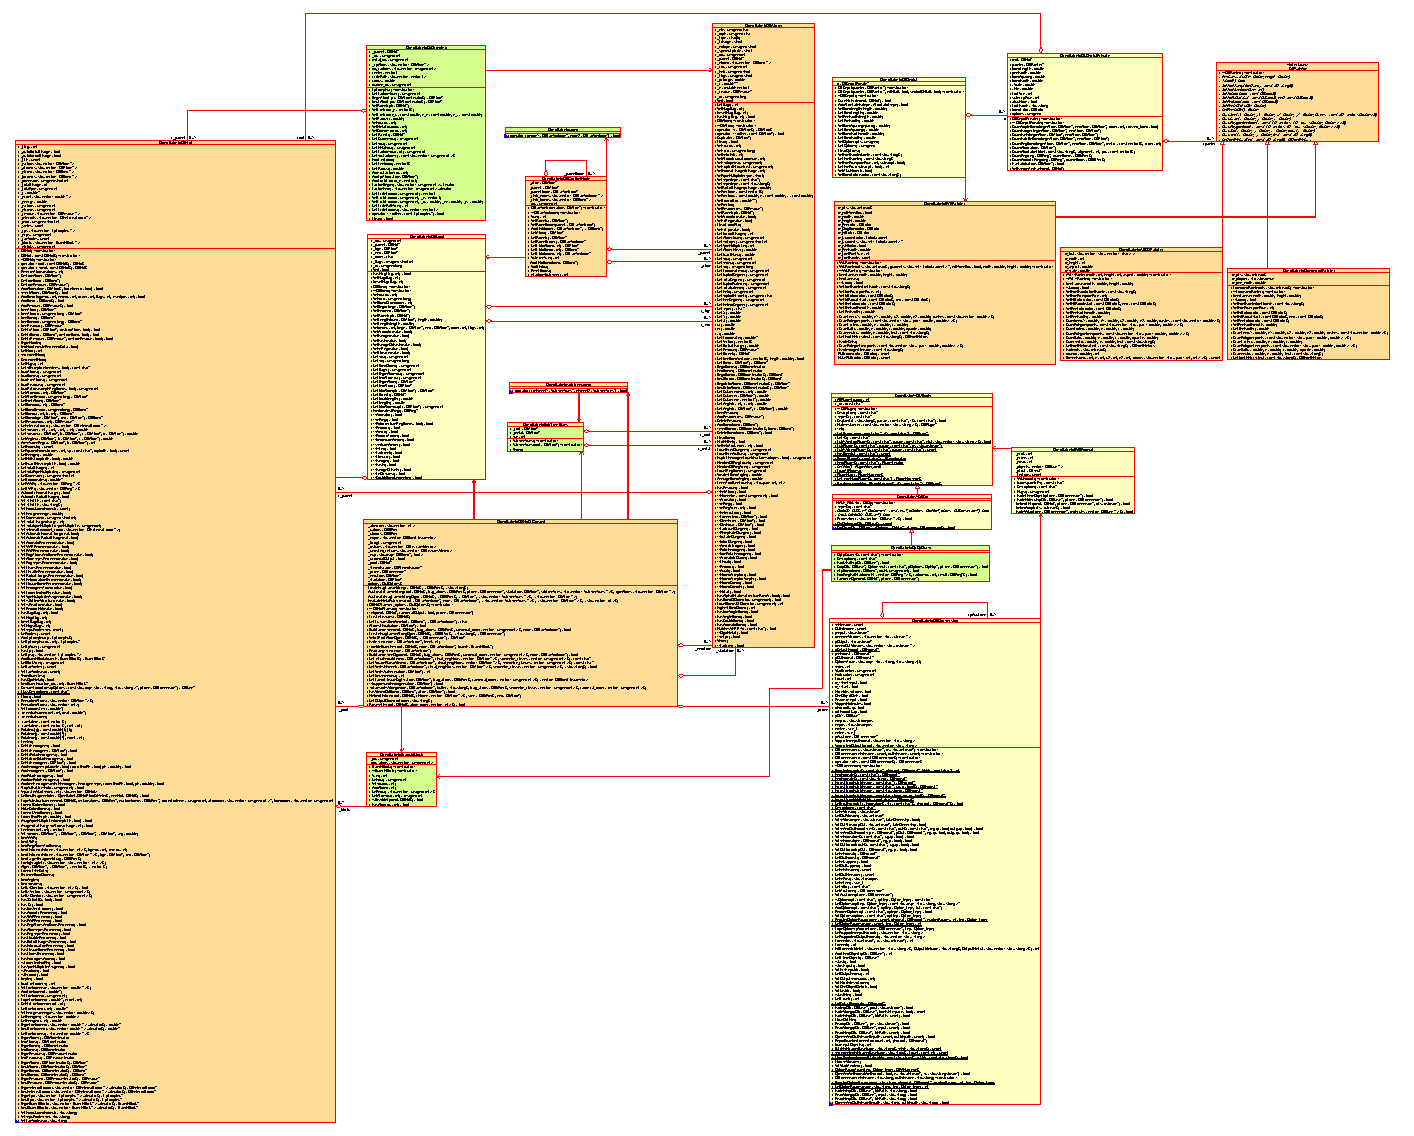
\includegraphics[scale=0.7]{imagenes/diseno/diagramaClasesHorizontal_cropped.pdf}
        \caption{Diagrama de clases}
        \label{fig:diagrama_clases}
    \end{figure}
\end{landscape}

% 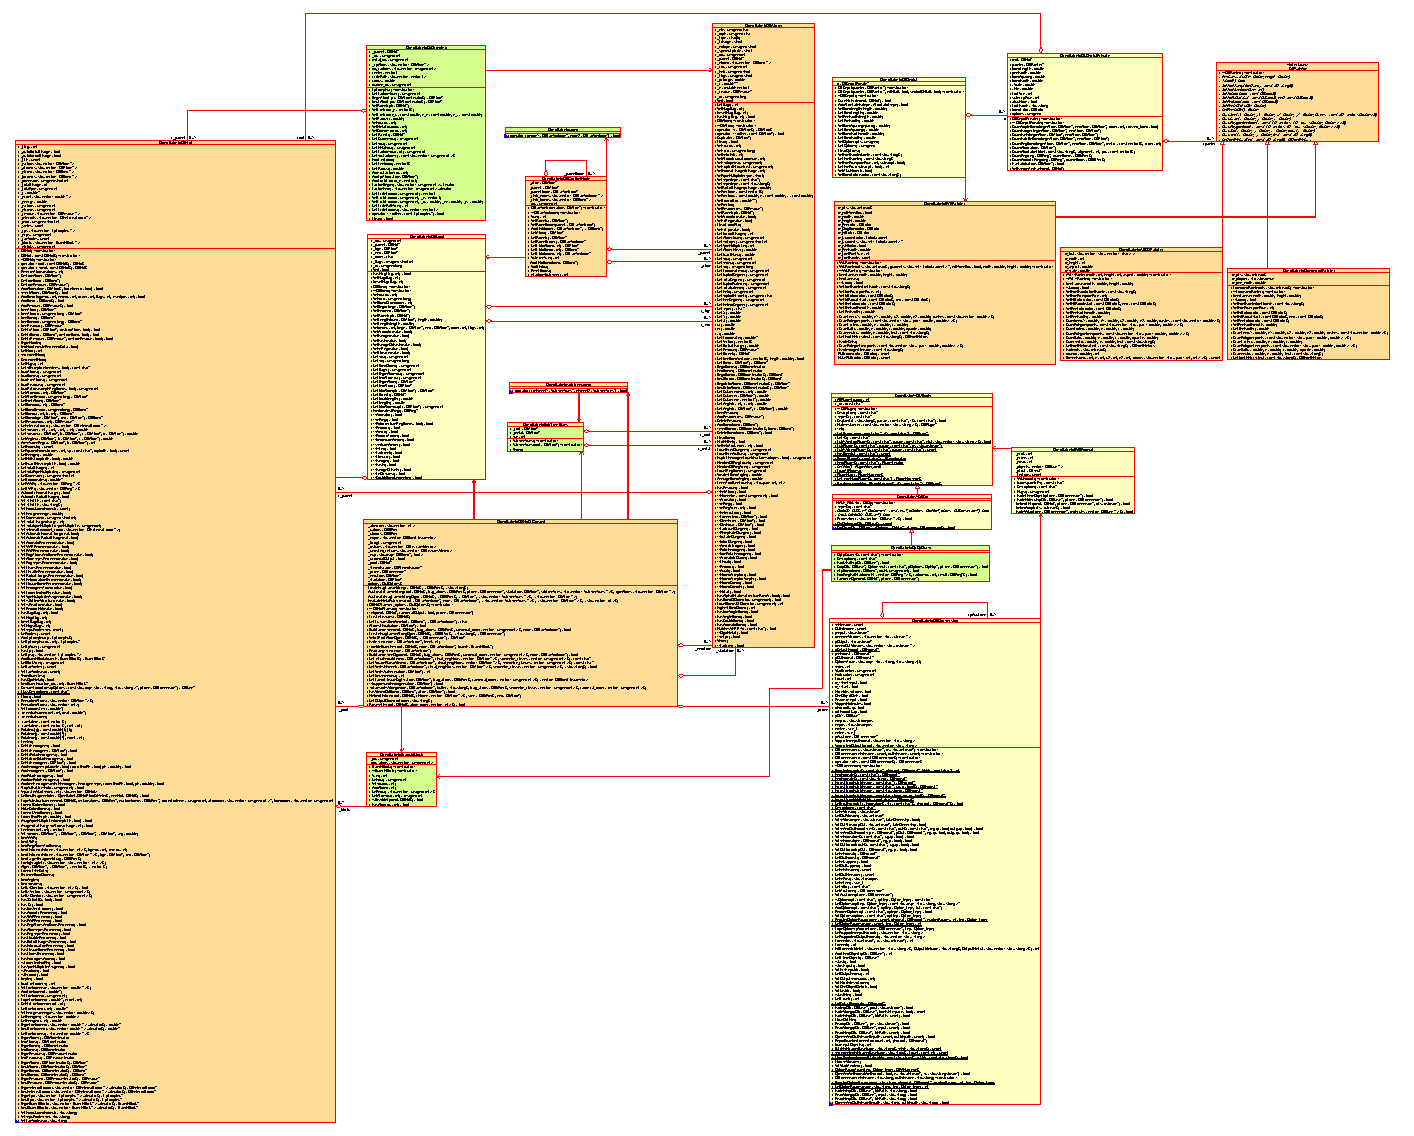
\includepdf[pages=-, offset=0 0,landscape=true,]{imagenes/diseno/diagramaClasesHorizontal_cropped.pdf}


Se pasa a detallar ahora cada una de ellas, tanto las modificadas como las nuevas, para qué sirven, y en qué consisten sus métodos brevemente. Las clases que no se han alterado, al igual que el resto de clases que no se incluyen en el diagrama se puede consultar su documentación en la página oficial \footnote{\url{https://openbabel.github.io/api/3.0/index.shtml}}. Puntualizar que existe una enorme cantidad de clases en la librería de OpenBabel, no tendería sentido añadirlas todas en el diagrama. Además, no todas poseen de documentación, por lo que la mayoría no aparecerán en la página anterior.

\section{Clases modificadas}
\begin{itemize}
    \item \textbf{OBPainter}: clase base abstracta para las clases de representación gráfica 2D. Se han añadido el siguiente método para poder utilizarlo en las clases que implementan esta interfaz:
    \begin{lstlisting}[language=C++]
        public: 
    
virtual void DrawPolygonLine(const std::vector<std::pair<double, double> >& points) = 0;
    \end{lstlisting}

    \item \textbf{SVGPainter}: clase que hereda de OBPainter y genera representaciones 2D en el formato de gráficos vectoriales SVG.
    \begin{lstlisting}[language=C++]
        public: 
    
//Inserts the necessary xml code in the .svg output file to draw a polygon according to the vector of points specified by @p points
void DrawPolygonLine(const std::vector<std::pair<double, double> >& points);
    \end{lstlisting}

    \item \textbf{ASCIIPainter}: clase que hereda de OBPainter.
    \begin{lstlisting}[language=C++]
        public: 
    
//The method is declared empty to avoid compilation errors due to interface implementation. It has no use 
void DrawPolygonLine(const std::vector<std::pair<double, double> >& points);
    \end{lstlisting}

    \item \textbf{CommandPainter}: clase que hereda de OBPainter.
    \begin{lstlisting}[language=C++]
        public: 
    
//The method is declared empty to avoid compilation errors due to interface implementation. It has no use 
void DrawPolygonLine(const std::vector<std::pair<double, double> >& points);
    \end{lstlisting}

    % -------------------------- Atom ---------------------------
    \item \textbf{OBAtom}: clase central, contiene la información relativa a un átomo. Se han añadido los siguientes métodos:
    \begin{lstlisting}[language=C++]
    public: 
    
//\return Is this a metal commonnly present in organometallic compounds?
bool IsOgmMetal();

//\return Is atom part of a Cp ring?
bool IsInCp() const;

//\return Is this atom a Carbon (atomic number == 6)?
bool IsCarbon();

//Debug method. Displays on basic output simple data to identify the atom
void Show();

//Mark an atom as part of a Cp ring
void SetInCp(bool value = true);
    \end{lstlisting}


    % -------------------------- Mol ---------------------------
    \item \textbf{OBMol}: clase central, almacena toda la información básica relacionada con una molécula. Se han añadido las siguientes variables y métodos:
    \begin{lstlisting}[language=C++]
    private: 
    
std::string _smiles;                //!< Input smiles string for the molecule
std::vector<CpComplex*> _cps;       //!< Cp information
unsigned int _ncps;                 //!< Number of cps complexes detected
std::string  _canSmiles;            //!< Canonical smiles based on Ogm canonicalization
std::vector<BranchBlock*> _blocks;  //!< Branches information
unsigned int _nblocks;              //!< Number of blocks


    public: 
    
//! Set the input smiles string of this molecule to @p smi
void SetInputSmiles(std::string smi);

//! \return the input smiles string of this molecule
std::string GetSmiles();

//! Add a new CpComplex specified by @p cp
void AddCpComplex(CpComplex& cp);

//! \return the cp at index @p idx or NULL if none exists.
CpComplex* GetCpComplex(int idx);

//! \return number of cp in the molecule
unsigned int GetCpSize();

//! \return whether the molecule has cps or not
bool HasCp();

//! \return the whole container of cps of this molecule
std::vector<CpComplex*> GetCps();

//! Add a new block to the molecule, specified by @p branch
BranchBlock* AddBranchBlock(BranchBlock& branch);

//! \return the number of blocks in the molecule
unsigned int GetBlockSize();

//! \return the canonical smiles string generated by the ogm canonicalization methods
std::string GetCanSmiles();

//! Set the canonical smiles string of this molecule to @p smi
void   SetCanSmiles(std::string smi);

//! Debug method. Displays on basic output all molecule blocks with basic information of the atoms.
void ShowBranches();

//! \return If this molecule has any Ogm metal or not
bool HasOgmMetal();

//! \return the block of which the carbon at index @p carbon_idx is part, or NULL if no such block exists
BranchBlock* FindBranch(int carbon_idx);

//! Set the iterator to the beginning of the Cp list
//! \return the first Cp structure, or NULL if none exist
CpComplex* BeginCp(std::vector<CpComplex*>::iterator & i);

//! Advance the iterator to the next Cp record
//! \return the next first Cp record, or NULL if none exist
CpComplex* NextCp(std::vector<CpComplex*>::iterator& i);

//! Set the iterator to the beginning of the BranchBlock list
//! \return the first BranchBlock structure, or NULL if none exist
BranchBlock* BeginBranchBlock(std::vector<BranchBlock*>::iterator& i);

//! Advance the iterator to the next BranchBlock record
//! \return the next first BranchBlock record, or NULL if none exist
BranchBlock* NextBranchBlock(std::vector<BranchBlock*>::iterator& i);
    \end{lstlisting}


    % -------------------------- OBMol2Cansmi ---------------------------
    \item \textbf{OBMol2Cansmi}: clase que maneja la conversión del smiles de entrada a un smiles canónico. Se han añadido los siguientes métodos:
    \begin{lstlisting}[language=C++]
        private: 
    
//Only changed visibility to private, since CreateFragCansmiStringOgm was created. Selects the "root" atom, which will be first in the SMILES, then builds a tree in canonical order, and finally generates the SMILES.
void CreateFragCansmiString(OBMol&, OBBitVec&, std::string&);

    
//Auxiliary private methods for SelectRootAtomOgm

//Shortened version of the CreateCansmiString method. Create the necessary variables to call AuxCreateFragCansmiStringOgm.
void AuxCreateCansmiString(OBMol& mol, OBBitVec& frag_atoms, OBConversion* pConv, OBAtom* startatom, std::vector<SubTreeSizes*>& subtreeSizes, std::vector<OBAtom*> ogmAtoms);

//Shortened version of the CreateFragCansmiStringOgm method. Create the necessary variables to build a new canonical tree using as root @p startAtom
void AuxCreateFragCansmiStringOgm(OBMol&, OBBitVec&, OBAtom*, std::vector<SubTreeSizes*>&, std::vector<OBAtom*>);

//Once the tree is built, this method runs through it in DFS evaluating the subtrees hanging from the other ogm metals. Use the auxiliary struct SubTreeSizes for this. 
void EvaluateMetalSubTrees(OBCanSmiNode* root, OBCanSmiNode* node, std::vector<SubTreeSizes*>&, std::vector<OBAtom*>&, std::vector<int>&);

        public: 
//Method based on CreateFragCansmiString. Share much of the code, with some additional methods specifically for my own canonical form designed for organometallic molecules.
void CreateFragCansmiStringOgm(OBMol&, OBBitVec&, std::string&, OBConversion*);

//If more than 1 Ogm metal is present in the molecule, this method chooses one of them, based on some rules and the conectivity of the metal within the molecule and the rest of the atoms
OBAtom* SelectRootAtomOgm(OBMol&, OBConversion*);

//Debug method for writing in basic output the tree with hierarchy formating
void WriteTree(OBCanSmiNode* node, int level = 0);

//Adds information to the molecule of the blocks that form it. Being a block, each set of atoms that, due to their bonds, are within the same parenthesis in the original input Smiles. Or, according to the OBMol2Cansmi::BuildCanonTree method, the parent-child relationship between atoms.
void IdentifyBranches(OBMol& mol,OBCanSmiNode* node, BranchBlock* branch = nullptr);

//Modifies the tree built by BuildCanonTree based on the length of the branches identified in IdentifyBranches. This is a canonical rule designed for a little more consistency in the output canon smiles.
void RearrangeTree(OBCanSmiNode* node);

//Builds the SMILES tree, in canonical order, for the specified molecular fragment. Based on the BuildCanonTree method. Shares much of the code, with some changes in the neighbour selection algorithm.
bool BuildCanonTreeOgm(OBMol& mol, OBBitVec& frag_atoms, vector<unsigned int>& canonical_order, OBCanSmiNode* node);
    \end{lstlisting}


    % -------------------------- OBCanSmiNode ---------------------------
    \item \textbf{OBCanSmiNode}: clase que representa un nodo. En conjunto se forma una estructura de árbol, cada nodo es un átomo del árbol para luego escribir el SMILES canónico. Se han añadido los elementos:
    \begin{lstlisting}[language=C++]
        private: 
    
OBCanSmiNode* _parentNode;      //!< Pointer to the parent node

//! Add a child bond to the node, specified by @p bond. Should only be used in the ResetBonds method as a part of the OBMol2Cansmi::RearrangeTree algorithm.
//! Otherwise, use addChildnode to add both the child node and its respective bonds
void AddChildBond(OBBond* bond);

        public: 

//! Set the parent node to @p parent
void SetParentNode(OBCanSmiNode* parent);

//! \return the parent node
OBCanSmiNode* GetParentNode();

//! Traverses the tree in dfs from the node calling the method
//! \return the number of total children (counting himself) 
int SubTreeSize();

//! Sort a node's child_nodes using a std::sort operation an a custom comparator 'mycomp'
void SortChilds();

//! When added at the same time in the addchildnode method, the child with its bond have a 1 to 1 index correspondence. When reordering the children, in OBMol2Cansmi::RearrangeTree, the indices of the bonds are lost. This method clears and adds the bonds back in order.
void ResetBonds();

//! \return the total number of carbons in this node subtree
int nCarbonsSubTree();
    \end{lstlisting}

\end{itemize}





\section{Clases nuevas}
\begin{itemize}
    % -------------------------- CpComplex ---------------------------
    \item \textbf{CpComplex}: clase que maneja y permite almacenar estructuras de ciclopentadienilo. Se han creado las siguientes variables y métodos:
    \begin{lstlisting}[language=C++]
	protected:
  
OBMol* _parent;                         //!< Parent molecule
unsigned int _idx;                      //!< Cp identifier within the molecule
unsigned int metal_idx;                 //!< Atom idx of central metal
std::vector<OBAtom*> _cpAtoms;          //!< Atoms for the carbons of the Cp structure
std::vector<unsigned int> idx_carbons;  //!< Atom indexes for the carbons of the Cp structure
vector3 center;                         //!< Cp center, for normal bond connection with metal atom, and aromatic circle position
std::vector<vector3> circlePath;        //!< Coordinates for the cp circle (needed to achieve a perspective circunference)
double radius;                          //!< Cp's aromatic circle radius
unsigned int dummy_idx;                 //!< Dummy central atom idx


        public:

//! Default constructor 
CpComplex();

//! \name Methods to modify internal information
//@{
//! Attach an OBMol @p ptr as the parent container for this Cp
void SetParent(OBMol* ptr);
//! Set the center point of the Cp, sprecified by @p _v. It is equidistant to every carbon in th Cp, as they are disposed in a regular polygon
void SetCentroid(vector3& _v);
//! Set the center point of the Cp, sprecified by @p v_x, v_y, v_z. It is equidistant to every carbon in th Cp, as they are disposed in a regular polygon
void SetCentroid(const double v_x, const double v_y, const double v_z);
//! Set the radius of the Cp circle
void SetRadius(double r);
//! Set the Cp identifier
void SetIdx(int idx);
//! Set the idx of the central metal to which this Cp is attached
void SetMetalIdx(int midx);
//! Dummy atom is created to make a perpendicular bond between the metal and the Cp drawing
//! Set the atom idx of the dummy atom created for this Cp 
void SetDummyIdx(int idx);
//! Set the point of the Cp circle at index @p i to the coordinates specified by @p _v
void SetCircleCoord(unsigned int i, vector3 _v);
//! Set the point of the Cp circle at index @p i to the coordinates specified by @p _vx, _vy, _vz
void SetCircleCoord(unsigned int i, double _vx, double _vy, double _vz = 0.0);
//@}


//! \name Methods to retrieve information
//@{
//! \return number of carbon atoms in the cp
unsigned int GetCarbonsSize();
//! \return the molecule which contains this Cp, or NULL if none exists
OBMol* GetParent();
//! \return dummy atom idx for this Cp structure, or 0 if none exists
unsigned int GetDummyIdx() const;
//! \return Cp identifier
unsigned int GetIdx() const;
//! \return Central metal identifier
unsigned int GetMetalIdx() const;
//! \return carbon idx at position @p i in tha container. Zero based access method to vector
unsigned int GetCarbonIdx(int i) const;
//! \return the whole contanier of carbon idx
const std::vector<unsigned int>& GetIdxCarbons();
//! \return the centroid of this Cp in a coordinate vector
vector3& GetCentroid();
//! \return the radius of the Cp circle
double GetRadius();
//! \return the coordinate vector for the Cp circle point at position @p i in the container. Zero based access method to vector
vector3 GetCircleCoord(unsigned int i);
//! \return the number of points of the Cp circle
int GetCirclePathSize() const;
//! \return the whole container of coordinates of the Cp circle
std::vector<vector3> GetCircleCoords() const;
//@}


//! \name Addition of data for a Cp
//@{
//! Adds a new atom idx to this Cp
void AddIdxCarbon(int idx);
//! Adds a new atom to this Cp
void AddCpAtom(OBAtom* atom);
//! Adds a new point to the coordinate vector that forms the Cp circle
void AddCircleCoord(vector3 _v);
//@}


//! \name Iteration methods
//@{
//! Set the iterator to the beginning of the Cp atom list
//! \return the first atom, or NULL if none exist
OBAtom* CpComplex::BeginAtomCp(OBAtomIterator& i);
//! Advance the iterator to the next atom in the Cp
//! \return the next first atom record, or NULL if none exist
OBAtom* CpComplex::NextAtomCp(OBAtomIterator& i);
//@}


//! \name Other operations
//@{
//! Calculate and set the centroid of this Cp, taking into consideration all atoms stored in _cpAtoms
void FindCentroid();
//! Equivalence operator
bool operator==(const CpComplex* other) const;
//@}




    \end{lstlisting}


    % -------------------------- BranchBlock ---------------------------
    \item \textbf{BranchBlock}: clase que representa un bloque definido dentro de la molécula, p.ej. un ciclo de benceno, un Cp, o toda una rama de un átomo. Se han añadido las siguientes variables y métodos:
    \begin{lstlisting}[language=C++]
        private: 
    
unsigned int _idx;                          //!< Block identifier
std::vector<unsigned int> vidx_atoms;       //!< Vector idx of the atoms that are part of the block.

        public: 

//! Default constructor
BranchBlock();

//! Destructor
~BranchBlock();

//! \return the size of the block (number of atoms in the block)
int Size();

//! \return the block identifier
unsigned int GetIdx();

//! Set the block identifier
void SetIdx(int idx);

//! Add an atom's idx to the block
void AddAtom(int i);

//! \return the idx of the atom at position @p i. Zero based access.
unsigned int GetAtomIdx(int i);

//! \return Whether the @p idx exists within the atoms already inserted in the block
bool HasAtom(int idx);

//! Cp will be possible if all the elements in the block are carbons up to that point and have a bond with an ogm metal.
//! \return whether or not it appears to be a Cp block
bool IsPossibleCp(OBMol &mol)
    \end{lstlisting}


    % -------------------------- OpCpDraw ---------------------------
    \item \textbf{OpCpDraw}: clase plugin que hereda de OBOp. Contiene el algoritmo de detección, identificación, y almacenamiento en la molécula de estructuras tipo Cp.
    \begin{lstlisting}[language=C++]

//! Default constructor
OpCpDraw(const char* ID);

//! Inherited method. 
//! Display through the output stream a brief description of the plugin.
const char* Description();

//! Inherited method. 
//! \return true if this op (plugin operation) is designed to work with the class of @p pOb, e.g. OBMol
virtual bool WorksWith(OBBase* pOb) const;

//! Inherited method. Required function that does the work. Normally return true, unless object is not to be output. 
virtual bool Do(OBBase* pOb, const char* OptionText = nullptr, OpMap* pOptions = nullptr, OBConversion* pConv = nullptr);

//! \return If @p bond is likely to be a cp-bond like
bool isCpBond(OBBond* bond, unsigned int idxM);

//! Finds the ring of which the carbon with idx @p carbonIdx is a part of, among the rings of @p rlist (obtained from a SSSR perspective), and stores it in @p result.
//! \returns whether it was found or not
bool FindRingWithCarbon(vector<OBRing*>& rlist, int carbonIdx, OBRing*& result);

//! Canonize the input SMILES and identify blocks
void CanonizeOgm(OBMol* mol, OBConversion* pConv); 
    \end{lstlisting}


    
    % -------------------------- SubTreeSizes ---------------------------
    \item \textbf{SubTreeSizes}: struct auxiliar creado para la selección del primer metal durante la canonización (se profundiza sobre esto en la sección \ref{reglas_canonizado}). Contiene las siguientes variables y métodos:
    \begin{lstlisting}[language=C++]

OBAtom* _root;      //!< Tree root
OBAtom* _metal;     //!< Metal to evaluate
int size;           //!< Size of the subtree for the _metal to evaluate

//! Default constructor
SubTreeSizes();

//! Parameter constructor. Creates a new object with _root as @p root
SubTreeSizes(OBAtom* root);

//! Debug method. Displays through basic output the struct information.
void Show();
    \end{lstlisting}


    % -------------------------- subtreecomp ---------------------------
    \item \textbf{subtreecomp}: objeto comparador que prioriza unos metales sobre otros en el proceso de selección del átomo raíz para el árbol (más en detalle en la Sección \ref{canonizacion}).
    \begin{lstlisting}[language=C++]
bool operator() (SubTreeSizes* element1, SubTreeSizes* element2) const;
    \end{lstlisting}


    % -------------------------- mycomp ---------------------------
    \item \textbf{mycomp}: objeto comparador que prioriza las ramas del árbol canónico durante el proceso de reordenación.
    \begin{lstlisting}[language=C++]
bool operator() (OBCanSmiNode* node1, OBCanSmiNode* node2);
    \end{lstlisting}


\end{itemize}






















\chapter{Experimentación}

Aquí la idea es ir poniendo las pruebas que vaya haciendo de las moléculas, y lo que vaya descubriendo. Problablemente exponer aqui tb el método o reglas de canonizacion a las que llegue.

% \input{capitulos/Conclusiones.tex}

% El nocite* es para que muestre todos los elementos de la bibliografia, aunque no se hayan usado para citar nada en el documento (usando \cite{})
% \nocite{*}
\printbibliography[title={Bibliografía}]
% \printbibliography{sample.bib}
% \printbibliography[type=online, title={Otras fuentes}]

% \printbibheading
% \printbibliography{nottype=misc, heading=subbibliography, title={Citas}}
% \printbibliography{type=misc, heading=subbibliography, title={Otras fuentes}}


% \nocite{*}
% \bibliography{sample}
% \bibliographystyle{ieeetr}
% \addcontentsline{toc}{chapter}{Bibliografía}
% \bibliographystyle{miunsrturl}
%


% ----------------------------------Apéndices-----------------------------
\appendix
\chapter{Tabla comparativa del set completo de moléculas}
\label{apend:pagina_tabla_intro_grande}

Para no hacer la tabla comparativa más grande de lo que ya es, se indican aquí los nombres de las moléculas junto con un identificador. Este identificador se usa a lo largo del documento en varias ocasiones para hacer referencia a estos nombres.

\begingroup
\renewcommand{\arraystretch}{1.5}

\begin{longtable}{cp{11cm}}
\caption{Tabla de índices con los nombres de las moléculas de la Tabla \ref{tabla:tabla_grande_apendice}}\\
    \hline
\textbf{Id} & \textbf{Nombre del compuesto} \\ \hline
\endfirsthead

\multicolumn{2}{c}%
{{\bfseries \tablename\ \thetable{} -- Continuación de la página anterior}} \\
\hline
 \textbf{Id} & \textbf{Nombre del compuesto} \\ \hline
\endhead

\hline \multicolumn{2}{r}{{Continúa en la siguiente página}} \\
\endfoot

\hline
\endlastfoot

1 & Methyl(triphenylphosphine)gold(I)  \\
%\hline
 2 & trans-Dibromobis(triphenylphosphine)palladium(II) \\
%\hline
 3 & Dichloro(1,5-cyclooctadiene)palladium(II) \\
%\hline
 4 & SK-CC 01A \\
%\hline
 5 & Bis[\textmu-chloro[5-hydroxy-2-[1-(hydroxyimino)ethyl]phenyl]palladium] \\
%\hline
 6 & (SP-4-3)-(3,5-Dichloro-2,4,6-trifluorophenyl)iodobis (triphenylarsine)palladium \\
%\hline


 7 & Palladium,(2,2\textquotesingle-bipyridine-\textit{k}N1,\textit{k}N1\textquotesingle)[(2,2-dimethyl-1,2-ethanediyl)-1,2-phenylene]fluoro(4-methylbenzenesulfonamidato-\textit{k}N)-, (OC-6-35)  \\
%\hline
 8 & Dibromo(1,2-dimethoxyethane)nickel(II) \\
%\hline
 9 & Bis(triphenylphosphine)ruthenium(II) dicarbonyl chloride \\
%\hline
 10 & Chloro(trimethylphosphine)gold(I) \\
%\hline
 11 & Chloro[tris(para-trifluoromethylphenyl)phosphine]gold(I) \\
%\hline
 12 & Chloro(dimethylsulfide)gold(I) \\
%\hline

 13 & Chloro(methyldiphenylphosphine)gold(I)  \\
%\hline
 14 & Chloro[diphenyl(o-tolyl)phosphine]gold(I) \\
%\hline
 15 & Chloro[(1,1\textquotesingle-biphenyl-2-yl)di-tert-butylphosphine]gold(I) \\
%\hline
 16 & (Acetonitrile)[(2-biphenyl)di-tert-butylphosphine] gold(I)hexafluoroantimonate \\
%\hline
 17 & Chloro[2-di-tert-butyl(2\textquotesingle,4\textquotesingle,6\textquotesingle-triisopropylbiphenyl)phosphine] gold(I) \\
%\hline
 18 & Chloro[2-dicyclohexyl(2\textquotesingle,4\textquotesingle,6\textquotesingle-trisopropylbiphenyl)phosphine]gold(I) \\
%\hline

 19 & BisPhePhos XD gold(I) chloride  \\
%\hline
 20 & Chloro[di(1-adamantyl)-2-dimethylaminophenylphosphine]gold(I) \\
%\hline
 21 & Dichloro(DPPE)digold(I) \\
%\hline
 22 & Dichloro[($\pm$)-BINAP]digold(I) \\
%\hline
 23 & Bis(chlorogold(I)) [1,1\textquotesingle-bis(diphenylphosphino)ferrocene] \\
%\hline
 24 & [(IMes)AuCl] \\
%\hline

 25 & [(IPr)AuCl]  \\
%\hline
 26 & IPrAuNTf2 \\
%\hline
 27 & DPPF \\
%\hline
 28 & Dicarbonylcyclopentadienyliodoiron(II) \\
%\hline
 29 & (OC-6-11\textquotesingle)-Bis[2,6-di(2-pyridinyl-\textit{k}N)phenyl-\textit{k}C]iron\\
 %\hline
30 & Chloro[5-methoxy-2-[1-[(4-methoxyphenyl)imino-\textit{k}N]ethyl]phenyl-\textit{k}C][(1,2,3,4,5-$\eta$)-1,2,3,4,5-pentamethyl-2,4-cyclopentadien-1-yl]iridium \\
%\hline
31 & Diiodo(pentamethylcyclopentadienyl)iridium(III) dimer
 \label{tabla:tabla_indices_apendice}
\end{longtable}

\endgroup




\begin{landscape}

% \small
\begin{longtable}{m{0.3cm}m{6.7cm}m{7.7cm}m{2.3cm}m{2.3cm}}
\caption{Tabla extendida para el set de datos de 30 moléculas. Contiene la cadena SMILES extraída de Sigma-Aldrich (SA), la cadena SMILES extraída de SciFinder (SF), y las imágenes de las respectivas bases de datos (SA y SF)}\\
\hline
 \textbf{Id} & \textbf{SMILES SA} & \textbf{SMILES SF} & \textbf{Imagen SA} & \textbf{Imagen SF} \\ \hline
\endfirsthead

\multicolumn{5}{c}%
{{\bfseries \tablename\ \thetable{} -- Continuación de la página anterior}} \\
\hline
\textbf{Id} & \textbf{SMILES SA} & \textbf{SMILES SF} & \textbf{Imagen SA} & \textbf{Imagen SF} \\ \hline
\endhead

\hline \multicolumn{5}{r}{{Continúa en la siguiente página}} \\
\endfoot

\hline
\endlastfoot

% Compuesto 2 del excel
 1 &
 C[Au].c1ccc(cc1)P(c2ccccc2) c3ccccc3 & 
 [Au+]([CH3-])[P](C=1C=CC=CC1) (C=2C=CC=CC2)C=3C=CC=CC3 & 
 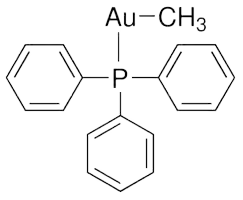
\includegraphics[width=2.2cm]{imagenes/sigmaAldrich/Methyl(triphenylphosphine)gold(I).png} & 
 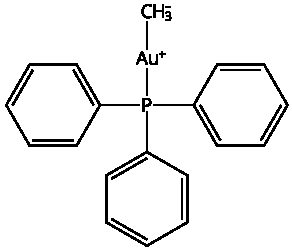
\includegraphics[width=2.2cm]{imagenes/sciFinder/pdf/Methyl(triphenylphosphine)gold(I).pdf} \\
%\midrule

% Compuesto 3 del excel
 2 &
 Br[Pd]Br.c1ccc(cc1) P(c2ccccc2)c3ccccc3.c4ccc(cc4) P(c5ccccc5)c6ccccc6 & 
 [Br-][Pd+2]([Br-])([P](C=1C= CC=CC1)(C=2C=CC=CC2) C=3C=CC=CC3)[P](C=4C=CC=CC4) (C=5C=CC= CC5)C=6C=CC=CC6 & 
 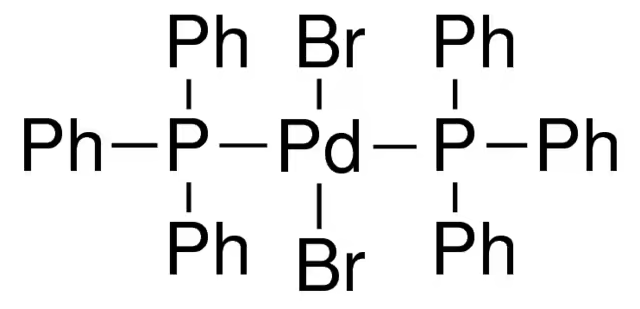
\includegraphics[width=2.2cm]{imagenes/sigmaAldrich/trans-Dibromobis(triphenylphosphine)palladium(II).png} & 
 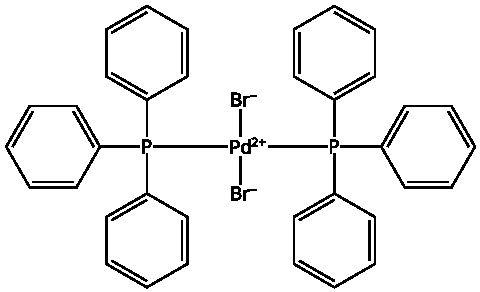
\includegraphics[width=2.2cm]{imagenes/sciFinder/pdf/trans-Dibromobis(triphenylphosphine)palladium(II).pdf} \\
%\midrule

% Compuesto 4 del excel
 3 &
 Cl[Pd]Cl.C1CC=CCCC=C1 & 
 [Cl-][Pd+2]123([Cl-]) [CH]=4CC[CH]3=[CH]2CC[CH]41 & 
 \includegraphics[width=2.2cm]{imagenes/sigmaAldrich/Dichloro(1,5-cyclooctadiene)palladium(II).png} & 
 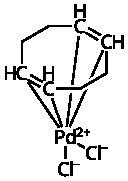
\includegraphics[width=2.2cm]{imagenes/sciFinder/pdf/Dichloro(1,5-cyclooctadiene)palladium(II).pdf} \\
%\midrule

% Compuesto 5 del excel
 4 &
 C1C[C@@H]2C[C@H]1CC2PC3C [C@@H]4CC[C@H]3C4.CN(C)c5ccccc5-c6ccccc6[Pd]Cl & 
 [Cl-][Pd+2]1([C-]=2C=CC=CC2C=3C =CC=CC3[N]1(C)C)[PH] (C4CC5CCC4C5)C6CC7CCC6C7 & 
 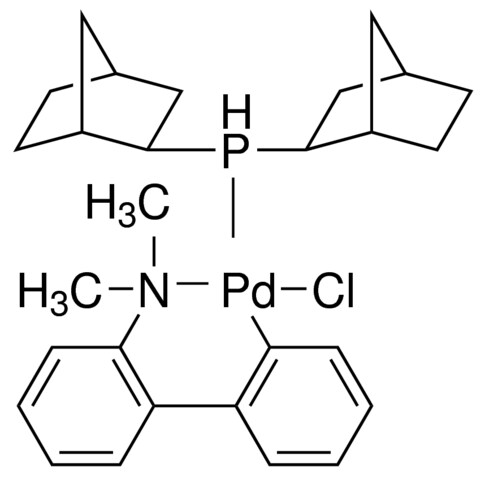
\includegraphics[width=2.1cm]{imagenes/sigmaAldrich/SK-CC 01A.jpeg} & 
 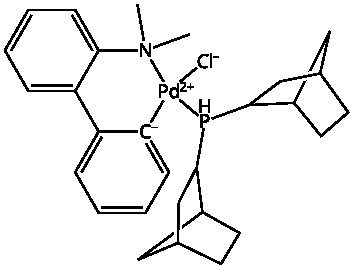
\includegraphics[width=2.2cm, height=2.1cm]{imagenes/sciFinder/pdf/SK-CC 01A.pdf} \\
%\midrule

% Compuesto 6 del excel
 5 &
 C\textbackslash C(=N/O)c1ccc(O)cc1[Pd]Cl .C\textbackslash C(=N/O)c2ccc(O)cc2[Pd]Cl & 
 OC=1C=CC=2C(=[N](O)[Pd+2]3 ([Cl-][Pd+2]4([Cl-]3)[C-]=5 C=C(O)C=CC5C(=[N]4O)C)[C-]2C1)C & 
 \includegraphics[width=2.2cm]{imagenes/sigmaAldrich/Bis[µ-chloro[5-hydroxy-2-[1-(hydroxyimino)ethyl]phenyl]palladium].jpeg} & 
 \includegraphics[width=2.2cm]{imagenes/sciFinder/pdf/Bis[µ-chloro[5-hydroxy-2-[1-(hydroxyimino)ethyl]phenyl]palladium].pdf} \\
%\midrule

\\ %Filas vacias para dar mas espacio entre el texto


% Compuesto 7 del excel
 6 &
 No se encontró el compuesto en Sigma-Aldrich & 
 FC=1C(Cl)=C(F)[C-](=C(F)C1Cl)[Pd+2] ([I-])([As](C=2C=CC=CC2)(C=3C=CC=C C3)C=4C=CC=CC4)[As](C=5C=CC=CC5) (C=6C=CC=CC6)C=7C=CC=CC7 & 
 & 
 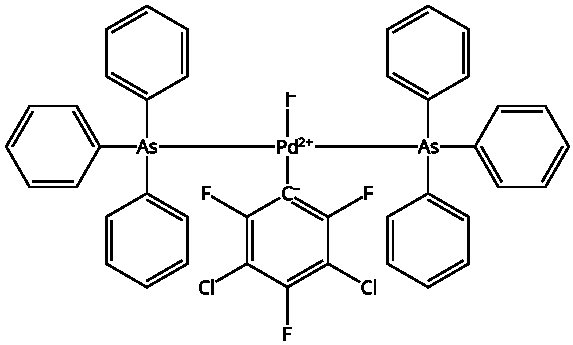
\includegraphics[width=2.5cm]{imagenes/sciFinder/pdf/(SP-4-3)-(3,5-Dichloro-2,4,6-trifluorophenyl)iodobis(triphenylarsine)palladium.pdf} \\
%\midrule

\\ %Filas vacias para dar mas espacio entre el texto

% Compuesto 8 del excel
 7 &
 No se encontró el compuesto en Sigma-Aldrich & 
 O=S(=O)([NH-][Pd+4]12([F-])([C-]=3C=CC=CC3C(C)(C)[CH2-]1) [N]=4C=CC=CC4C=5C=CC=C[N] 52)C6=CC=C(C=C6)C & 
 & 
 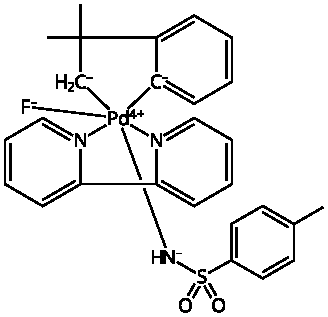
\includegraphics[width=2.2cm]{imagenes/sciFinder/pdf/Palladium, (2,2-bipyridine-κN1,κN1)[(2,2-dimethyl-1,2-ethanediyl)-1,2-phenylene]fluoro(4-methylbenzenesulfonamidato-κN)-, (OC-6-35).pdf} \\
%\midrule


% Compuesto 9 del excel
 8 &
 Br[Ni]Br.COCCOC & 
 [Br-][Ni+2]1([Br-])O(C)CCO1C & 
 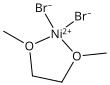
\includegraphics[width=2.2cm]{imagenes/sigmaAldrich/Nickel(II) bromide ethylene glycol dimethyl ether complex.png} & 
 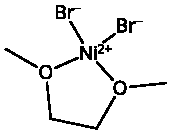
\includegraphics[width=2.2cm]{imagenes/sciFinder/pdf/Dibromo(1,2-dimethoxyethane)nickel(II).pdf} \\
%\midrule


% Compuesto 10 del excel
 9 &
 Cl[Ru](Cl)(C\#[O])(C\#[O])([PH](c1ccc cc1)(c2ccccc2)c3ccccc3)[PH](c4ccc cc4)(c5ccccc5)c6ccccc6 & 
 O\#C[Ru+2]([Cl-])([Cl-])(C\#O)([P](C=1C=CC=CC1) (C=2C=CC=CC2)C=3C=CC=CC3)[P] (C=4C=CC=CC4)(C=5C=CC=CC5) C=6C=CC=CC6 & 
 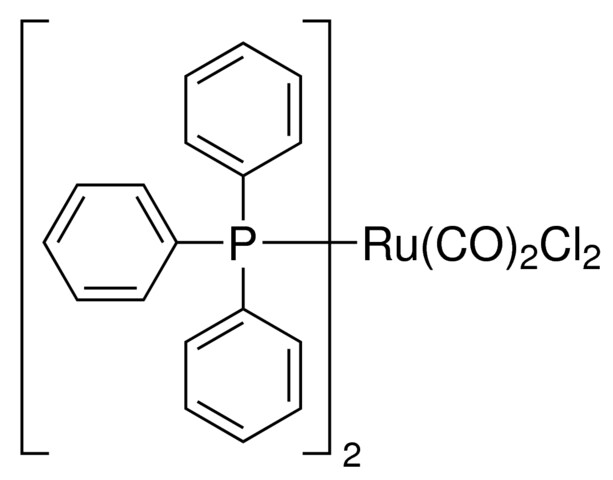
\includegraphics[width=2.2cm]{imagenes/sigmaAldrich/Bis(triphenylphosphine)ruthenium(II) dicarbonyl chloride.jpeg} & 
 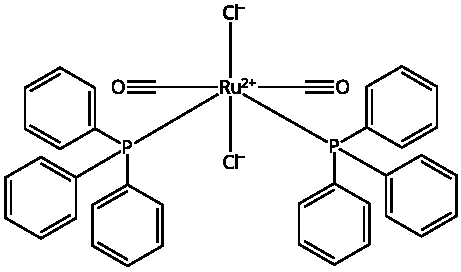
\includegraphics[width=2.2cm]{imagenes/sciFinder/pdf/Bis(triphenylphosphine)ruthenium(II) dicarbonyl chloride.pdf} \\
%\midrule

% Compuesto 11 del excel
 10 &
 Cl[Au].CP(C)C & 
 [Cl-][Au+][P](C)(C)C & 
 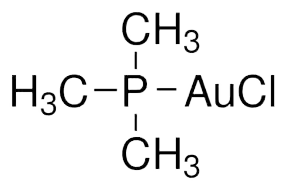
\includegraphics[width=2.2cm]{imagenes/sigmaAldrich/Chloro(trimethylphosphine)gold(I).png} & 
 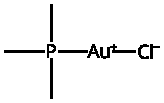
\includegraphics[width=2.2cm]{imagenes/sciFinder/pdf/Chloro(trimethylphosphine)gold(I).pdf} \\
%\midrule


% Compuesto 12 del excel
 11 &
 Cl[Au].FC(F)(F)c1ccc(cc1)P(c2ccc (cc2)C(F)(F)F)c3ccc(cc3)C(F)(F)F & 
 FC(F)(F)C1=CC=C(C=C1)[P] ([Au+][Cl-])(C2=CC=C(C=C2)C(F) (F)F)C3=CC=C(C=C3)C(F)(F)F & 
 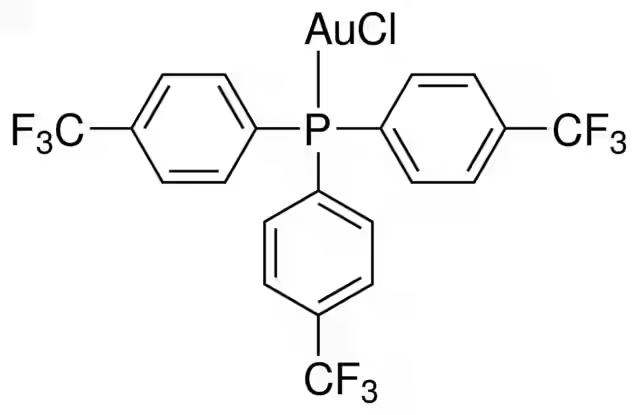
\includegraphics[width=2.2cm]{imagenes/sigmaAldrich/Chloro[tris(para-trifluoromethylphenyl)phosphine]gold(I).png} & 
 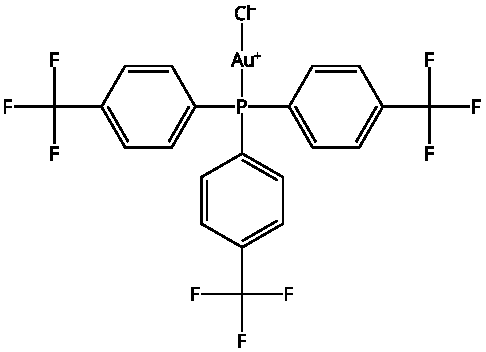
\includegraphics[width=2.2cm]{imagenes/sciFinder/pdf/Chloro[tris(para-trifluoromethylphenyl)phosphine]gold(I).pdf} \\
%\midrule



% Compuesto 13 del excel
 12 &
 Cl[Au].CSC & 
 [Cl-][Au+][S](C)C & 
 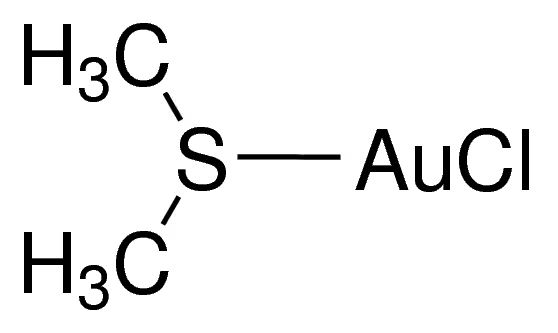
\includegraphics[width=2.2cm]{imagenes/sigmaAldrich/Chloro(dimethylsulfide)gold(I).png} & 
 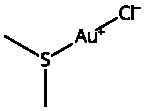
\includegraphics[width=2.2cm]{imagenes/sciFinder/pdf/Chloro(dimethylsulfide)gold(I).pdf} \\
%\midrule



% Compuesto 14 del excel
 13 &
 Cl[Au].CP(c1ccccc1)c2ccccc2 & 
 [Cl-][Au+][P](C=1C=CC=CC1) (C=2C=CC=CC2)C & 
 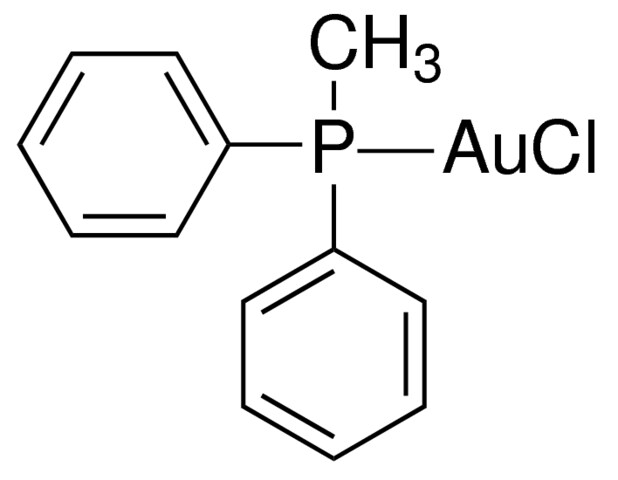
\includegraphics[width=2.1cm, height=1.5cm]{imagenes/sigmaAldrich/Chloro(methyldiphenylphosphine)gold(I).jpeg} & 
 \includegraphics[width=2.2cm]{imagenes/sciFinder/pdf/Chloro(methyldiphenylphosphine)gold(I).pdf} \\
%\midrule




% Compuesto 15 del excel
 14 &
 Cl[Au].Cc1ccccc1P(c2ccccc2)c3ccccc3 & 
 [Cl-][Au+][P](C=1C=CC=CC1) (C=2C=CC=CC2)C=3C=CC=CC3C & 
 \includegraphics[width=2.2cm]{imagenes/sigmaAldrich/Chloro[diphenyl(o-tolyl)phosphine]gold(I).jpeg} & 
 \includegraphics[width=2.2cm]{imagenes/sciFinder/pdf/Chloro[diphenyl(o-tolyl)phosphine]gold(I).pdf} \\
%\midrule


% Compuesto 16 del excel
 15 &
 Cl[Au].CC(C)(C)P(c1ccccc1-c2ccccc2)C(C)(C)C & 
 [Cl-][Au+][P](C=1C=CC=CC1C=2C =CC=CC2)(C(C)(C)C)C(C)(C)C & 
 \includegraphics[width=2.2cm]{imagenes/sigmaAldrich/Chloro[(1,1-biphenyl-2-yl)di-tert-butylphosphine]gold(I).png} & 
 \includegraphics[width=2.2cm]{imagenes/sciFinder/pdf/Chloro[(1,1-biphenyl-2-yl)di-tert-butylphosphine]gold(I).pdf} \\
%\midrule



% Compuesto 17 del excel
 16 &
 [Au+].CC\#N.F[Sb-](F)(F)(F)(F)F. CC(C)(C)P(c1ccccc1-c2ccccc2)C(C)(C)C & 
 [F-][Sb+5]([F-])([F-])([F-])([F-])[F-]. C(\#[N][Au+][P](C=1C=CC=CC1C= 2C=CC=CC2)(C(C)(C)C)C(C)(C)C)C & 
 \includegraphics[width=2.2cm]{imagenes/sigmaAldrich/(Acetonitrile)[(2-biphenyl)di-tert-butylphosphine]gold(I) hexafluoroantimonate.jpeg} & 
 \includegraphics[width=2.2cm]{imagenes/sciFinder/pdf/(Acetonitrile)[(2-biphenyl)di-tert-butylphosphine]gold(I) hexafluoroantimonate [1compuesto].pdf} \\
  &  &  &  &
 \includegraphics[width=2.2cm]{imagenes/sciFinder/pdf/(Acetonitrile)[(2-biphenyl)di-tert-butylphosphine]gold(I) hexafluoroantimonate [2compuesto].pdf} \\
%\midrule



% Compuesto 18 del excel
 17 &
 CC(C)c1cc(C(C)C)c(c(c1)C(C)C)-c2 ccccc2[PH]([Au]Cl)(C(C)(C)C)C(C)(C)C & 
 [Cl-][Au+][P](C=1C=CC=CC1C=2C (=CC(=CC2C(C)C)C(C)C)C(C)C)(C(C) (C)C)C(C)(C)C & 
 \includegraphics[width=2.2cm]{imagenes/sigmaAldrich/Chloro[2-di-tert-butyl(2,4,6-triisopropylbiphenyl)phosphine] gold(I).jpeg} & 
 \includegraphics[width=2.3cm]{imagenes/sciFinder/pdf/Chloro[2-di-tert-butyl(2,4,6-triisopropylbiphenyl)phosphine] gold(I).pdf} \\
%\midrule



% Compuesto 19 del excel
 18 &
 Cl[Au].CC(C)c1cc(C(C)C)c(c(c1)C(C) C)-c2ccccc2P(C3CCCCC3)C4CCCCC4 & 
 [Cl-][Au+][P](C=1C=CC=CC1C=2C (=CC(=CC2C(C)C)C(C)C)C(C)C)(C3C CCCC3)C4CCCCC4 & 
 \includegraphics[width=2.2cm]{imagenes/sigmaAldrich/Chloro[2-dicyclohexyl(2,4,6-trisopropylbiphenyl)phosphine]gold(I).png} & 
 \includegraphics[width=2.2cm]{imagenes/sciFinder/pdf/Chloro[2-dicyclohexyl(2,4,6-trisopropylbiphenyl)phosphine]gold(I).pdf} \\
%\midrule

\\ %Filas vacias para dar mas espacio entre el texto

% Compuesto 20 del excel
 19 &
 CC(C)OC(C=CC=C1OC(C)C)=C1C2 =CC(P(C3CCCCC3)C4=CC(C5=C(O C(C)C)C=CC=C5OC(C)C)=CC=C4) =CC=C2.[Au]Cl & 
 [Cl-][Au+][P](C=1C=CC=CC1C2=C(OC(C) C)C=CC=C2OC(C)C)(C=3C=CC=CC3C4 =C(OC(C)C)C=CC=C4OC(C)C)C5CCCCC5 & 
 \includegraphics[width=2.2cm]{imagenes/sigmaAldrich/pdf/BisPhePhos XD gold(I) chloride.pdf} & 
 \includegraphics[width=2.2cm]{imagenes/sciFinder/pdf/BisPhePhos XD gold(I) chloride.pdf} \\
%\midrule



% Compuesto 21 del excel
 20 &
 Cl[Au].CN(C)c1ccccc1P(C23C C4CC(CC(C4)C2)C3)C56CC7CC(C C(C7)C5)C6 & 
 [Cl-][Au+][P](C=1C=CC=CC1N (C)C)(C23CC4CC(CC(C4)C2)C3) C56CC7CC(CC(C7)C5)C6 & 
 \includegraphics[width=2.2cm]{imagenes/sigmaAldrich/Chloro[di(1-adamantyl)-2-dimethylaminophenylphosphine]gold(I).png} & 
 \includegraphics[width=2.2cm]{imagenes/sciFinder/pdf/Chloro[di(1-adamantyl)-2-dimethylaminophenylphosphine]gold(I).pdf} \\
%\midrule





% Compuesto 22 del excel
 21 &
 Cl[Au].Cl[Au].C(CP(c1ccccc1) c2ccccc2)P(c3ccccc3)c4ccccc4 & 
 [Cl-][Au+][P](C=1C=CC=CC1) (C=2C=CC=CC2)CC[P]([Au+][Cl-]) (C=3C=CC=CC3)C=4C=CC=CC4 & 
 \includegraphics[width=2.2cm]{imagenes/sigmaAldrich/Dichloro(DPPE)digold(I).jpeg} & 
 \includegraphics[width=2.2cm]{imagenes/sciFinder/pdf/Dichloro(DPPE)digold(I).pdf} \\
%\midrule


% Compuesto 23 del excel
 22 &
 Cl[Au].Cl[Au].P(C1=CC=CC=C1)(C2 =C(C3=C(C=CC4=C3C=CC=C4)P (C5=CC=CC=C5)C6=CC=CC=C6)C7 =C(C=CC=C7)C=C2)C8=CC=CC=C8 & 
 [Cl-][Au+][P](C=1C=CC=CC1)(C=2C =CC=CC2)C3=CC=C4C=CC=CC4=C3 C=5C=6C=CC=CC6C=CC5[P]([Au+] [Cl-])(C=7C=CC=CC7)C=8C=CC=CC8 & 
 \includegraphics[width=2.2cm]{imagenes/sigmaAldrich/Dichloro[(±)−BINAP]digold(I).png} & 
 \includegraphics[width=2.2cm]{imagenes/sciFinder/pdf/Dichloro[(±)−BINAP]digold(I).pdf} \\
%\midrule


% Compuesto 24 del excel
 23 &
 [Fe].Cl[Au].Cl[Au].[CH]1[CH] [CH][C]([CH]1)P(c2ccccc2)c3 ccccc3.[CH]4[CH][CH][C]([CH]4) P(c5ccccc5)c6ccccc6 & 
 [Cl-][Au+][P](C=1C=CC=CC1)(C=2C=CC =CC2)[C-]34[CH]5=[CH]6[CH]7=[CH]3[Fe+2] 6789\%10\%1154[CH]=\%12[CH]\%11=[CH]\%10 [C-]9([CH]\%128)[P]([Au+][Cl-])(C=\%13 C=CC=CC\%13)C=\%14C=CC=CC\%14 & 
 \includegraphics[width=2.5cm]{imagenes/sigmaAldrich/pdf/Bis(chlorogold(I)) [1,1-bis(diphenylphosphino)ferrocene.png} & 
 \includegraphics[width=2.2cm]{imagenes/sciFinder/pdf/Bis(chlorogold(I)) [1,1-bis(diphenylphosphino)ferrocene].pdf} \\
%\midrule


% Compuesto 25 del excel
 24 &
 Cl[Au].Cc1cc(C)c(N2[C]N(C=C2) c3c(C)cc(C)cc3C)c(C)c1 & 
 Cl[Au]=C1N(C=CN1C=2C(=CC(=CC2 C)C)C)C=3C(=CC(=CC3C)C)C & 
 \includegraphics[width=2.2cm]{imagenes/sigmaAldrich/pdf/[(IMes)AuCl].pdf} & 
 \includegraphics[width=2.2cm]{imagenes/sciFinder/pdf/[(IMes)AuCl].pdf} \\
%\midrule


% Compuesto 26 del excel
 25 &
 CC(C)c1cccc(C(C)C)c1N2C=CN(C2 [Au]Cl)c3c(cccc3C(C)C)C(C)C & 
 Cl[Au]=C1N(C=CN1C=2C(=CC=CC2C (C)C)C(C)C)C=3C(=CC=CC3C(C)C)C(C)C & 
 \includegraphics[width=2.2cm]{imagenes/sigmaAldrich/[(IPr)AuCl].png} & 
 \includegraphics[width=2.2cm]{imagenes/sciFinder/pdf/[(IPr)AuCl].pdf} \\
%\midrule

% Compuesto 27 del excel
 26 &
 CC(C)c1cccc(C(C)C)c1N2C=CN(C2= [Au]N(S(=O)(=O)C(F)(F)F)S(=O) (=O)C(F)(F)F)c3c(cccc3C(C)C)C(C)C & 
 O=S(=O)(N([Au]=C1N(C=CN1C=2C(= CC=CC2C(C)C)C(C)C)C=3C(=CC=CC3C (C)C)C(C)C)S(=O)(=O)C(F)(F)F)C(F)(F)F & 
 \includegraphics[width=2.1cm]{imagenes/sigmaAldrich/IPrAuNTf2.png} & 
 \includegraphics[width=2.2cm]{imagenes/sciFinder/pdf/IPrAuNTf2.pdf} \\
%\midrule

% Compuesto 29 del excel
 27 &
 [Fe].[CH]1[CH][CH][C]([CH]1)P (c2ccccc2)c3ccccc3.[CH]4[CH][CH] [C]([CH]4)P(c5ccccc5)c6ccccc6 & 
 C=1C=CC(=CC1)P(C=2C=CC=CC2) [C-]34[CH]5=[CH]6[CH]7=[CH]3[Fe+2] 6789\%10\%1154[CH]=\%12[CH]\%11= [CH]\%10[C-]9(P(C=\%13C=CC=CC\%13) C=\%14C=CC=CC\%14)[CH]\%128 & 
 \includegraphics[width=2.2cm]{imagenes/sigmaAldrich/DPPF.png} & 
 \includegraphics[width=2.2cm]{imagenes/sciFinder/pdf/DPPF.pdf} \\
%\midrule

% Compuesto 30 del excel
 28 &
 [Fe]I.[C-]\#[O+].[C-]\#[O+]. [CH]1[CH][CH][CH][CH]1 & 
 O\#C[Fe+2]1234([I-])(C\#O)[CH]= 5[CH]4=[CH]3[CH-]2[CH]51 & 
 \includegraphics[width=2.2cm]{imagenes/sigmaAldrich/Dicarbonylcyclopentadienyliodoiron(II).png} & 
 \includegraphics[width=2.2cm]{imagenes/sciFinder/pdf/Dicarbonylcyclopentadienyliodoiron(II).pdf} \\
%\midrule

% Compuesto 31 del excel
 29 &
 No se encontró el compuesto en Sigma-Aldrich & 
 C=1C=C[N]2=C(C1)C3=CC=CC=4C=5C= CC=C[N]5[Fe+2]672([C-]34)[C-]=8C(=CC=CC8C=9C=CC=C [N]96)C=\%10C=CC=C[N]\%107 & 
 & 
 \includegraphics[width=2.2cm]{imagenes/sciFinder/pdf/(OC-6-11)-Bis[2,6-di(2-pyridinyl-κN)phenyl-κC]iron.pdf}\\
%\midrule

% Compuesto 32 del excel
 30 &
 [CH]1[CH][CH][CH][CH]1.COc2ccc (cc2)\textbackslash N=C(/C)c3ccc(OC)cc3[Ir]Cl & 
 [Cl-][Ir+3]12345([C-]6=CC(OC)=C C=C6C(=[N]1C=7C=CC(OC)=C C7)C)C=8(C)C5(C)=C4(C)[C-]3(C)C82C & 
 \includegraphics[width=2.2cm]{imagenes/sigmaAldrich/iridio_solo.png} & 
 \includegraphics[width=2.2cm]{imagenes/sciFinder/iridio_solo.png}\\
%\midrule

% Compuesto 33 del excel
 31 &
 I[Ir]I.I[Ir]I.C[C]1[C](C)[C](C)[C](C) [C]1C.C[C]2[C](C)[C](C)[C](C)[C]2C & 
 [I-][Ir+3]12345([I-][Ir+3]6789([I-])([I-]1)C=\%10(C)C9(C)=C8(C)[C-]7(C)C \%106C)C=\%11(C)C5(C)=C4(C) [C-]3(C)C\%112C & 
 \includegraphics[width=2.2cm]{imagenes/sigmaAldrich/iridio_doble.png} & 
 \includegraphics[width=2.2cm]{imagenes/sciFinder/iridio_doble.png}
% \hline
\label{tabla:tabla_grande_apendice}

\end{longtable}

\end{landscape}




\chapter{Manual de usuario}
\label{apend:manual}

Aquí la idea es describir los procesos de instalacion de las herramientas mas importantes del proyecto, siendo, la instalacion y buildeado local de openbabel, y la instalacion de visual studio c++, y como utilizarlo para añadir nuevos ficheros al proyecto ya existente y ejecutar obabel por linea de comandos para generar resultados.




%%\input{apendices/paper/paper}
%\input{glosario/entradas_glosario}
% \addcontentsline{toc}{chapter}{Glosario}
% \printglossary
% \chapter*{}
\thispagestyle{empty}

\end{document}